%
% This text file include all filess neccessary to create
% the User's Guide
%

%====== define a new class for layout

\documentclass[a4paper]{../covise}


%====== set some useful packages for HTML, color, graphics, longer table
%====== floating text around images , pdf-links ...

\usepackage{html, htmllist}
\usepackage{hyperref}
\usepackage{graphicx}
\usepackage{longtable}

%\usepackage{palatino}
%\renewcommand{\familydefault}{\sfdefault}


\setlength\LTleft{0pt}
\setlength\LTright\fill


%====== start the documentclass


\begin{document}


%====== the following tables are only used by PS/PDF
%====== also the titlepage and the next page
\begin{latexonly}

\begin{titlepage}
    \setcounter{page}{0}
	 \thispagestyle{empty}
    \unitlength1cm
    
       \begin{picture}(15,17)
       \put(2, -2.5){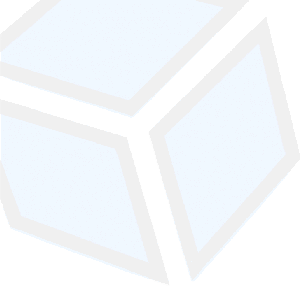
\includegraphics[scale=5]{../visenso_title}}     
       \put(0,-3){\line(1,0){15}}
       \put(0, 10){\makebox(15,2)[t]{\Huge{COVISE}}}
       \put(0, 9){\makebox(15,2)[t]{\Huge{Installation and Configuration}}}
       \put(0, 8){\makebox(15,2)[t]{\LARGE{July 2005}}}   
       \end{picture}
    
	\newpage
   \setcounter{page}{0}
	\thispagestyle{empty}
   \uppertitleback{\bf{Title:} \\
			COVISE  \\ 
			Installation and Configuration \\
         \today }
   \vfill
	\lowertitleback{\bf{Authors:} \\
         Daniela Rainer}

\end{titlepage}


\pagenumbering{arabic}
\tableofcontents
%	\listoffigures
%	\listoftables
	
\end{latexonly}



%====== include the chapters

\begin{htmlonly}

\usepackage{html, htmllist}
\usepackage{longtable}

\bodytext{bgcolor="#ffffff" link="#0033cc" vlink="#0033cc"}

%%%==================================================	
%%%==================================================	

% #1  mark defined by \label
% #2  a linktext 
% #3  a html link 
\newcommand{covlink}[3]{\htmladdnormallink{#2}{#3} \latex{(\ref{#1})} }


\newenvironment{covimg}[4]%
{
 \begin{figure}[htp]
  \begin{center}
   \latexonly
      \includegraphics[scale=#4]{#1/pict/#2}
   \endlatexonly  
   \html{\htmladdimg[align="center"]{pict/#2.png}}
   \caption{#3}
  \end{center}
 \end{figure} 
}{} 

\newenvironment{covimg2}[3]%
{ 
 \begin{figure}[htp]
  \begin{center}
     \latexonly
       \includegraphics[scale=#3]{#1/pict/#2}   
     \endlatexonly
     \html{\htmladdimg[align="center"]{pict/#2.png}}
  \end{center}
 \end{figure} 
}{}

\definecolor{output}{rgb}{0.,0.,1.}
\definecolor{depend}{rgb}{1.,0.65,0.}
\definecolor{required}{rgb}{0.58,0.,0.83}
\definecolor{optional}{rgb}{0.,0.39,0.}

\newcommand{\addimage}[1] {\html{\htmladdimg{pict/#1.png}}}

\newcommand{\addpict}[4] {\latexonly
	     \begin{figure}[!htbp]
			  \begin{center}
   	 		  \includegraphics[scale=#1]{#2}
   	 		  \caption{#3}
		 		  \label{#4}
			  \end{center}
	 		\end{figure}
	     \endlatexonly}



\end{htmlonly}

%================================================================================
%================================================================================


%================================================================================
\startdocument

\chapter{Introduction}

OpenCOVER (OpenSceneGraph COvise Virtual Environment Renderer) is a COVISE renderer module
with support for Virtual Reality (VR) input devices, backprojection displays,
Augmented Reality and intuitive interaction. 
OpenCOVER can also be started independently of COVISE and just be used as a stand-alone collaborative virtual
reality viewer for 3D geometry.

This document explains how OpenCOVER is configured for your Virtual Environment. 
The section
\html{\htmladdnormallink{Graphics Board and Display}{../display/display.html}}\latex{{Graphics Board and Display}
   (\ref{label_chapter_display})} describes how to setup stereo and multiple screens.

The section
\html{\htmladdnormallink{Input Devices}{../input/input.html}}\latex{{Input Devices}
   (\ref{label_chapter_input})}
explains how the 3D input and tracking devices are configured.



\begin{htmlonly}

\usepackage{html, htmllist}
\usepackage{longtable}

\bodytext{bgcolor="#ffffff" link="#0033cc" vlink="#0033cc"}

%%%==================================================	
%%%==================================================	

% #1  mark defined by \label
% #2  a linktext 
% #3  a html link 
\newcommand{covlink}[3]{\htmladdnormallink{#2}{#3} \latex{(\ref{#1})} }


\newenvironment{covimg}[4]%
{
 \begin{figure}[htp]
  \begin{center}
   \latexonly
      \includegraphics[scale=#4]{#1/pict/#2}
   \endlatexonly  
   \html{\htmladdimg[align="center"]{pict/#2.png}}
   \caption{#3}
  \end{center}
 \end{figure} 
}{} 

\newenvironment{covimg2}[3]%
{ 
 \begin{figure}[htp]
  \begin{center}
     \latexonly
       \includegraphics[scale=#3]{#1/pict/#2}   
     \endlatexonly
     \html{\htmladdimg[align="center"]{pict/#2.png}}
  \end{center}
 \end{figure} 
}{}

\definecolor{output}{rgb}{0.,0.,1.}
\definecolor{depend}{rgb}{1.,0.65,0.}
\definecolor{required}{rgb}{0.58,0.,0.83}
\definecolor{optional}{rgb}{0.,0.39,0.}

\newcommand{\addimage}[1] {\html{\htmladdimg{pict/#1.png}}}

\newcommand{\addpict}[4] {\latexonly
	     \begin{figure}[!htbp]
			  \begin{center}
   	 		  \includegraphics[scale=#1]{#2}
   	 		  \caption{#3}
		 		  \label{#4}
			  \end{center}
	 		\end{figure}
	     \endlatexonly}



\end{htmlonly}

%================================================================================
%================================================================================


%================================================================================
\startdocument
\chapter{Graphics Board and Display}
\label{label_chapter_display}

VR Environments today come in various flavours  First you have to differentiate between head mounted displays (HMDs) and 
projection based virtual environments. Both types are supported by OpenCOVER.
For stereo you need either a graphics board which supports active stereo video
formats, such as NVIDIA Quadro boards, a graphics board with two video outputs, a computer with
two graphics boards or two computers connected to each other via a LAN.
Some display devices such as Autostereoscopic displays can be driven by a single graphics output by using interlaced
stereo modes. Some of those are also supported by OpenCOVER.
For driving more than one display device like in tiled displays or multiple screen projection environments, either a cluster of computers, 
multiple graphics boards in one computer or any combination of those are nedded.
The following sections explains which combinations are supported by OpenCOVER
and how they are configured.


\section{Virtual Environment Types with Fixed Screens}
\label{label_section_vetypes}

OpenCOVER supports all types of Virtual Environments (VEs) with spatially
fixed  planar screens like a CAVE, Powerwall, Workbench or Holobench.
The VEs differ in the number of screens, the number of people they are suited for
and the level of immersion.

A Powerwall is a semi-immersive system with one big flat translucent canvas. 
The image is projected from behind, so that people don't stand in the optical path
of the projector.
The resolution can be enhanced by composing the final image from several graphics
boards, video outputs or several computers. A Powerwall is well suited
for presentations for large groups. As the user is not completely surrounded by screens
the immersion is lost when he looks too far to the left or right, up or down.

A Workbench is a semi-immersive system with a single translucent canvas. 
The workbench dimensions are similar to a drawing board and often the screen 
can be tilted back.
The advantage of a workbench is, that
the user can reach every point on the screen. It is suitable for small groups 
(3-4 persons).
The stereo impression and therefore the immersion gets lost when objects 
in the scene are cut by the frame of the workbench.

\begin{covimg}{display}{workbench}{RUS Workbench}{0.4}\end{covimg}

The Visenso Cykloop is a mobile one-screen backprojection system
with a screen size of 160 x 120 cm.

\begin{covimg}{display}{cykloop}{Vircinity Cycloop}{0.4}\end{covimg}

A CAVE (TM) is a system where the walls form a cube. The first CAVE was 
built at EVL. There are CAVEs with 4 screens (left, front, right and bottom), with 5 screens, (additionally the ceiling)
and 6 screens. The more screens the CAVE has the better is the immersion. The dimension of
one cube side is typically 3000 mm x 3000 mm. A CUBE is suited for smaller number of persons up to six or eight.

\begin{covimg}{display}{cave}{RUS Cube}{0.4}\end{covimg}

A Holobench has two screens, a front and a bottom screen.
The bottom screen is on the height of a table and the dimensions are like the 
ones of a workbench.
A Holospace also has a front and a bottom screen, but the bottom screen
is on the floor and the dimensions are like a CAVE.

Tiled displays are monoscopic or autostereoscopic highres displays composed out of an array of flat pannel displays.

% TODO: missing file
%\begin{covimg}{display}{TiledDisplay}{Calit Varrier}{0.4}\end{covimg}

\section{Stereo Modes}
\label{label_section_stereo_modes}

To improve the immersion in the VE, COVER supports stereo. Stereo means
that two images are presented to the user, one computed from the
view of the left eye, and one computetd from the view of the right eye.
Stereo can be turned on or off by setting the Stereo value to "ON" or "OFF". The default is "OFF"!

\small \begin{verbatim}
<Stereo vaue="ON" />
\end{verbatim} \normalsize

The separation between the two eyes can be specified with separaton attribute in the Stereo entry. The actual distance between the eyes differs from human to human but
the default of 60 mm is good in most cases. If you want to disable stereo for taking pictures or a movie, you can temorarily disable the stereo separation in
the 3D GUI under View options or set this value to 0.  

\small \begin{verbatim}
<Stereo separation="60" />
\end{verbatim} \normalsize

Special glasses ensure that each eye sees only the appropriate image. 
As in natural viewing, the brain forms a 3D image from the two images
from two different perspectives.

There are several methods for stereo viewing: red-green stereo, interlaced stereo and most important: active and passive stereo.

\subsection{Active Stereo}
		
In active stereo, the graphics card of the computer needs to be able
to switch to a video mode, where the left and the right image are stored
in different areas of the video memory. Every video frame it
switches between the left and the right image. This mode is called QuadBuffer mode. Special
glasses called shutter glasses which can make the glass opaque are synchronised
with the graphics card trough an infrared emitter. When the graphics card
displays the left image, the right glass is set to opaque and vice versa.

\begin{covimg}{display}{shutterglasses}{Shutter Glasses and Infrared
Emitter}{0.7}\end{covimg}

This stereo mode is supported among others on NVIDIA Quadro boards and AMD/ATI FireGL boards as well as most SGI Systems.
In order to enable QuadBuffer Stereo, you have to modify the X-Configuration according to your driver's documentation.
On WindowsXP and Vista, you have to open your graphicsdriver controll pannel, go to 3D options and enable stereo.
On Linux systems, you have to modify your X configuration, typically located in /etc/X11/xorg.conf
for ATI boards you have to add the following to your xorg.conv:
\begin{samepage}
\small \begin{verbatim}
Option "Stereo" "on"
\end{verbatim} \normalsize
\end{samepage}

for NVIDIA boards you have to select an appropriate Stereo mode similar to the following line, see
/usr/share/doc/NVIDIA\_GLX-1.0/README.txt

\begin{samepage}
\small \begin{verbatim}
Option "Stereo" "3"
\end{verbatim} \normalsize
\end{samepage}
After restaring our X server, you can verify that your graphics board is in stereo mode by running "glxinfo".
In the output, there is a column called "st ro" (for stereo). Some of the lines have to contain a "y" in that column

\begin{samepage}
\small \begin{verbatim}
   visual  x  bf lv rg d st colorbuffer ax dp st accumbuffer  ms  cav
 id dep cl sp sz l  ci b ro  r  g  b  a bf th cl  r  g  b  a ns b eat
----------------------------------------------------------------------
0x21 24 tc  0 32  0 r  y  .  8  8  8  0  4 24  8 16 16 16 16  0 0 None
0x22 24 tc  0 32  0 r  y  y  8  8  8  0  4 24  8 16 16 16 16  0 0 None
0x23 24 tc  0 32  0 r  y  .  8  8  8  8  4 24  8 16 16 16 16  0 0 None
\end{verbatim} \normalsize
\end{samepage}

On SGI Maximum Impact and Infinite Reality Systems it is 
possible to switch between a mono and a stereo video format on the fly 
as longs as the "managed area" remains the same.

If you want to
switch the monitor into stereo only when COVER is running you can
specify the setmon command with the command attributes to the Stereo and Mono entry.

Example:

\begin{samepage}
\small \begin{verbatim}
<Stereo command="/usr/gfx/setmon -n 1024x768_96s" />
<Mono command="/usr/gfx/setmon -n 1280x1024_76" />	
\end{verbatim} \normalsize
\end{samepage}

With setmon only standard video formats can be loaded. Infinite 
Reality Systems support also custom video formats which can be loaded
with the command ircombine.
If the video mode should not be changed (for example because the correct mode is
already running all the time), set command to and empty string. (this is the default)

Finally, you have to select a stereo visual for rendering. you can do that with the stereo attribute in the appropriate Window Entry.

\begin{samepage}
\small \begin{verbatim}
<Window index="0" width="1280"height="1024" decoration="false" stereo="true" />	
\end{verbatim} \normalsize
\end{samepage}


\subsection{Passive Stereo}

In passive stereo the left and the right image are presented at the
same time, but at two different video outputs which are connected to
two projectors. Each projector has a polarised lense. 
Special stereo glasses with polarised glasses ensure that each eye
sees the appropriate image.

The application
typically opens two windows or one window with two viewports and
draws the left and right image into the separate windows/viewports.
Another possibility is that two different computers create the left
and the right image.

	  
\begin{covimg}{display}{polarizedglasses}{Polarized Glasses}{0.7}\end{covimg}

Passive stereo can be created either with a graphics board with two
video outputs or with two computers.

\paragraph{Passive stereo with two video outputs}
Most of today's graphics boards support two video
outputs (dual-head). On nvidia cards it is called TwinView. 
If the window manager supports the Xinerama mode, you can also configure
only one large window with two viewports aka channels. If not, you need to configure
two windows. The preferred choice is one large window with two
channels, because it needs less ressources (for example textures need
to be loaded to the graphics board only once).
On Linux, you can enable the second output of your graphics card by modifying you xorg.conf, see the following example:
note that you have to disable XineramaInfo, otherwise you can't open a single window which spans both screens.

\begin{samepage}
\small \begin{verbatim}
  Option      "TwinView" "true"
  Option      "ConnectedMonitor" "CRT-0, DFP-1"
  Option      "SecondMonitorHorizSync" "30-168"
  Option      "SecondMonitorVertRefresh" "50-60"
  Option      "MetaModes" "1280x1024,1400x1050x60.00"
  Option      "IgnoreEDID" "true"
  Option      "NoTwinViewXineramaInfo" "true"
\end{verbatim} \normalsize
\end{samepage}


On SGI system you need the "multichannel option", this means a graphics
board with more than one video output. SGI Infinite Reality systems
can have 2-8 video outputs.


\paragraph{Passive stereo with two computers}
COVER can also be configured to use two computers (nodes) to create one
(passive) stereo image. The computers need to be synchronised
either via a serial cable or via ethernet. 
A powerwall or a cave can be driven by any number of nodes. Typical combinations are one node per screen with a passive stereo dual head configuration per
node or one node per screen and per eye. The latter is the configuration with highest rendering performance.
 
2*n or 2*n+1 computers. In the 2n+1 mode one computer
can be used as controlling computer, where COVISE is started and
where the Mapeditor is running, the other 2*n computers are then used 
only for rendering. You can also have COVER on the controlling computer.
In case that the controlling computer doesn't have a COVER, you
have to start the tracker through the Vircinity Device Server (see chapter
Tracking and Input Devices). The tracking system is connected
only to the masterPC or the controlling computer. the tracking
information is sent to the other computers via the network.

This multi-PC mode is configured in covise.config in the section
MultiPC. Here you indicate which computer is the master and which are
the slaves. Each computer needs a screen, window and channel configuration
for mono mode. As one half of the computers need to draw a left image
and the other alf a right image, this has to be indicated:

\small 
\begin{verbatim}
MultiPC: <masterPC> <slavePC1> <slavePC2> <...>
{
    SyncMode          <TCP SERIAL>
    SyncProcess       <APP DRAW>
    SerialDevice      <device>
    Master            <masterPC>
    MasterInterface   <masterPC>
    Host0             <slavePC1>    
    Host1             <....>
    ...
    numSlaves         <n>
}

COVERConfig: <masterPC>
{
    TRACKING_SYSTEM             <tracking system>
    STEREO                      off
    MONO_VIEW                   <LEFT RIGHT MIDDLE>
}

COVERConfig: <slavePC>
{
    TRACKING_SYSTEM             NONE
    STEREO                      off
    MONO_VIEW                   <LEFT RIGHT MIDDLE>
}

\end{verbatim}
\normalsize



\subsection{Memory consumption in active stereo mode} 
The active stereo modes (also called quadbuffer stereo) need four framebuffers, 
front and back (for doublebuffering), left and right (for stereo). 

The minimum amount of frame buffer memory you can allocate per pixel is 256 bits (small). The
amount of memory you can allocate per pixel can be doubled (512 or medium) or quadrupled 
(1024 or large).

During configuring the framebuffer with ircombine you select the frame buffer depth.
When you choose deepest the maximum pixeldepth for your configuration is selected.

With the program 'findvis' you can then check which framebuffer configurations (visuals)
are possible with the selected pixeldepth. For example, the IR2 pipe at RUS, configured for medium pixel depth,
offers the following configuration:
\small 
\begin{verbatim}
0x6f, RGBA 12/12/12/12, db, stereo, Z 23, S 1, samples 4
\end{verbatim}
\normalsize

COVER requests a framebuffer configuration with RGBA, doublebuffer, stereo and multisampling.
If it can't get such a visual, it selects one, which matches some of the criteria, for
example multisampling, but not stereo.

In case you don't get a visual with multisampling and stereo, you can tell COVER
to forgo multisampling:
\small 
\begin{verbatim}
COVERConfig
{
    ...
    ANTIALIAS OFF
    ...
}
\end{verbatim}
\normalsize

On SGI IR systems on each raster manager you have 80 GB of video memory. Here some typical
workbench configurations and the respective framebuffer calculations:

\begin{description}

\item [1024x768, framebuffer medium]
1024*768*512 = 50.33 GB. This combination of resolution and framebuffer depth is
 possible with one RM.

\item [2048x768, framebuffer medium]
2048*768*512 = 100.66 GB. With a managed area of 2048x768 you could configure 
two video outputs, each with 1028x768.
As this combination of resolution and framebuffer depth needs
more than 80 GB, you would need a second RM.

\end{description}

For COVISE and COVER it is quite useful, to have two video outputs, a monitor where
you run the mapeditor and a Workbench, CAVE or Powerwall where you run COVER.

\section{Loading Video Formats on SGI systems}
On SGI systems different video formats can be loaded. All systems besides
IR support only a fixed number of formats. Stereo Formats
are available on SGI Impact (1024x768\_96s), VPro (1280x1024\_100s), RealityEngine
(1024x768\_96s) and
InfiniteReality graphics boards. On IR Systems custom video formats
can be created using the video format compiler. Generally,
video format files reside in the directory 
\begin{verbatim}
/usr/gfx/ucode/<boardname>/vof
\end{verbatim}
and have the extension .vfo.

Custom video formats have to be loaded using the program /usr/gfx/ircombine,
while the predefined formats can be loaded with /usr/gfx/setmon. Look at the
manpages of setmon for details.

On IR systems you can have more than one video output per pipe. This can be
used to drive more than 1 projector for example for a powerwall system,
or a cave, or for passive stereo. The two video otputs are configured
with ircombine. Select 2 channels, apply the appropriate video format
on each channel and save this a combination file (extension .cmb).
The frequencies of the video formats in one combination need to be either
the same or multiples. The resolution doesn't need to be the same. Look
at the manpages of ircombine for details.

\section{Multipipe Synchronisation on SGI IR systems}
\label{label_section_multipe_sync}

If you drive your VE with more than one pipe (this is possible with
SGI IR systems only), the pipes have to be synchronised. For
synchronising the vertical retrace of the pipes, you have to genlock
the pipes with the genlock cable. When you create the video combination
you have to indicate, which pipe is the master (synchronisation intern)
and which one is the slave (synchronisation extern).

For synchronising the buffer swap
there are two different possibilities: hardware and software. For the
hardware solution you have to connect the swap ready cable.

The buffer swap synchronisation mode needs to be indicated in the section
COVERConfig. The keyword is PIPE\_LOCKING and the possible modes are called
CHANNEL (hardware), or WINDOW (software). 

\section{Configuration}
\label{label_section_configuration}
COVER reads the file covise.config to configure the number of
graphics boards, windows, viewports etc..
The following sections explain how to congigure COVER for a your VE.

\subsection{Pipe configuration}
The entry NUM\_PIPES in the section COVERConfig defines how many graphics 
boards are used for the application. 
\small
\small \begin{verbatim}
COVERConfig
{
    ...
    NUM_PIPES	<number of graphics boards used for COVER>
    ...
}
\end{verbatim}
\normalsize
In the section PipeConfig for each pipe used in the application
the appropriate hardware pipe is defined.
\begin{samepage}
\small
\small \begin{verbatim}
PipeConfig
{
    <index> <screen> <:server.display>
    <index> <screen> <:server.display>
    ...
}
\end{verbatim}
\end{samepage}
\normalsize
In multipipe operation the pipes have to be synchronized. See section 3.1.4
for details on pipe synchronisation on SGI Onyx systems.

\subsection{Screen configuration}
 
The entry NUM\_SCREENS in the section COVERConfig defines the number of 
phsical screens/walls in this VE. A workbench has one screen, a holobench 
two screens, a CAVE four two six screens etc.
\small
\begin{verbatim}
COVERConfig
{	
    ...
    NUM_SCREENS	<number of screens>
    ...
}
\end{verbatim}
\normalsize
The section ScreenConfig defines the size, position and orientation
of each screen in relation to the world coordinate system. In a CAVE
the recommended origin of the wolrd coordinate system is in the
center of the cube, in a workbench or powerwall system the best choice
for the origin is the middle of the screen.
\small
\begin{verbatim}
ScreenConfig
{
    <index> <name> <width  [mm]> <height[mm]> <origin [mm]> <euler angles [degree]>
    <index> <name> <width  [mm]> <height[mm]> <origin [mm]> <euler angles [degree]>
    ...
}
\end{verbatim}
\normalsize
\subsection{Window Configuration}

The entry NUM\_WINDOWS defines the number of windows. Imagine a 
holobench: if the computer has only one graphics board but two video
outputs you can define one pipe, one window and two channels, if the computer
has two graphics board you can define 2 pipes and 2 windows.
\small
\begin{verbatim}
COVERConfig
{
    ...
    NUM_WINDOWS	<number of windows>
    ...
}
\end{verbatim}
\normalsize
In the section WindowConfig the location of the window (left bottom corner) 
on the managed area and the size is defined:

\small \begin{verbatim}
WindowConfig
{
    <index> <name> <pipe index> <origin [pixels]> <size [pixels]>
    <index> <name> <pipe index> <origin [pixels]> <size [pixels]>
    ...
}
\end{verbatim} \normalsize


\subsection{Channel Configuration}

The number of channels (= viewports) is the same as the number of screens.
In the section ChannelConfig the left, bottom, right and top of the 
viewport in fractions between 0 and 1 or the left bottom width and height
in pixels in relation to the the window is defined. 

\small \begin{verbatim}
ChannelConfig
{
    <index> <name> <window index> <left> <bottom> <right> <top>
    <index> <name> <window index> <left> <bottom> <right> <top>
    ...
}
\end{verbatim} \normalsize
\small \begin{verbatim}
ChannelConfig
{
    <index> <name> <window index> <left> <bottom> <width> <height>
    <index> <name> <window index> <left> <bottom> <width> <height>
    ...
}
\end{verbatim} \normalsize




\newpage
\section{Example Configurations}
\label{label_section_examples}

In the covise directory you find several example configuration
\begin{itemize}
\item covise.config.cave-astereo-4pipes-motionstar: 4-sided cave, active stereo, two graphics pipes
\item covise.config.cave-astereo-2pipes-motionstar:  4-sided active, stereo cave, four graphics pipes
\item covise.config.workbench-astereo-polhemus: Tilted Workbench, active stereo, 1 pipe
\item covise.config.cycloop-pstereo-1window-fob: Cykloop, passive stereo, 1 pipe, 1 window, 2 viewports
\item covise.config.cycloop-pstereo-2window-fob: Cykloop, passive stereo, 1 pipe, 2 window
\item covise.config.cycloop-2cluster-vrc: Cykloop, passive stereo, cluster of 2 computers
\item covise.config.cycloop-2+1cluster-vrc: Cykloop, passive stereo, cluster of 3 computers
 
\end{itemize}

\subsection{4-sided CAVE with active stereo}
\begin{covimg}{display}{ruscube_sketch}{Sketch of the RUS CUBE}{1.0}\end{covimg}

The images for the four projectors of the 4-sided CAVE in this example are generated 
by an SGI onyx with active stereo. The video formats are custom formats. 
The aspect ratio of the resolution 
matches the one of the wall dimensions. The left, front and right wall
have height=2800mm, width=2500mm, the floor dimesion is 2800mm x 2800mm.
The video format for the walls has 992x992 pixels with a frequency of 
114 Hz, the floor has 1024x992 pixels at 114 Hz.

If only two pipes are used for the cave, the managed area on the
wall-wall-pipe is 992x992, on the wall-bottom pipe 1024x992.
If all four pipes are used for the cave, the managed area resolution is
equal to the window resolution.


\subsection{Tilted workbench with active stereo}

The workbench is operated by an SGI Onyx with one pipe.
We configured a 
combination of two video channels each with the format 1024\_768\_96s. 
The managed area is 2048x768 with medium pixel depth. 
To the first video output we connected a normal monitor, to the second 
one the projector. Therefore the COVER window has its origin at [1024 0]
(see section WindowConfig).
 
The dimension of the screen is 1700 mm x  1270 mm, and the screen is 
tilted 40 degrees.

\begin{covimg}{display}{rusworkbench_sketch}{Sketch of the RUS Workbench}{0.9}\end{covimg}


\subsection{Cykloop with passive stereo}
\begin{covimg}{display}{cykloop_sketch}{Sketch of the Vircinity Cycloop}{1.0}\end{covimg}

The cycloop has two projectors, the passive stereo images can be either generated by one
computer with two video channels or by two synchronised computers. In case of one
computer the configuration of one large window with two viewports is  preferable, because
textures are loaded only once.
			% using COVER (Daniela Rainer)	
\begin{htmlonly}

\usepackage{html, htmllist}
\usepackage{longtable}

\bodytext{bgcolor="#ffffff" link="#0033cc" vlink="#0033cc"}

%%%==================================================	
%%%==================================================	

% #1  mark defined by \label
% #2  a linktext 
% #3  a html link 
\newcommand{covlink}[3]{\htmladdnormallink{#2}{#3} \latex{(\ref{#1})} }


\newenvironment{covimg}[4]%
{
 \begin{figure}[htp]
  \begin{center}
   \latexonly
      \includegraphics[scale=#4]{#1/pict/#2}
   \endlatexonly  
   \html{\htmladdimg[align="center"]{pict/#2.png}}
   \caption{#3}
  \end{center}
 \end{figure} 
}{} 

\newenvironment{covimg2}[3]%
{ 
 \begin{figure}[htp]
  \begin{center}
     \latexonly
       \includegraphics[scale=#3]{#1/pict/#2}   
     \endlatexonly
     \html{\htmladdimg[align="center"]{pict/#2.png}}
  \end{center}
 \end{figure} 
}{}

\definecolor{output}{rgb}{0.,0.,1.}
\definecolor{depend}{rgb}{1.,0.65,0.}
\definecolor{required}{rgb}{0.58,0.,0.83}
\definecolor{optional}{rgb}{0.,0.39,0.}

\newcommand{\addimage}[1] {\html{\htmladdimg{pict/#1.png}}}

\newcommand{\addpict}[4] {\latexonly
	     \begin{figure}[!htbp]
			  \begin{center}
   	 		  \includegraphics[scale=#1]{#2}
   	 		  \caption{#3}
		 		  \label{#4}
			  \end{center}
	 		\end{figure}
	     \endlatexonly}



\end{htmlonly}

%================================================================================
%================================================================================


%================================================================================
\startdocument

\chapter{Input Devices}
\label{label_chapter_input}
COVER supports headtracking and a tracked hand device with several buttons.
Headtracking means, that the position and orientation of the users head is
captured and used to compute an appropriate view on the scene. With the
tracked hand device the user can select and manipulate parts of the scene.

Supported tracking devices are the Polhemus FASTRAK (POLHEMUS), the 
Ascension Motionstar (MOTIONSTAR),
and the Ascension Flock of Birds (FOB). Additionally all devices supported by the
CAVELIB can be used if a trackerdeamon from CAVELIB is installed.
These tracking systems use electromagnetic
fields to determine the position and orientation of a remote object. 
The Polhemus FASTRAK and the Ascension Flock of Birds are connected to 
the serial port of the computer, the Ethernet Motionstar system is a PC
where each sensor is connected to an internal Motionstar receiver (ISA) card. The PC transmitts
the position and orientation data via ethernet to the graphics workstation.

The input devices mouse (SPACEPOINTER), the Spaceball (SPACEBALL), the Phantom (PHANTOM), 
the Flybox (COVER\_FLYBOX) and the Beebox (COVER\_BEEBOX) and 
can be used only for hand tracking.

The Ascension and Polhemus trackers can also be combined with other commercial or
selfmade button devices. Supported button devices are the ICIDO Mike (MIKE), the
division Joystick (DVISION), the CEREAL Box (CEREAL), the Virtual Presense  xxx 
(VIRTUAL\_PRESENCE), the Pinch Glove (PINCH) and all devices supported by cavelib.

%-----

\section{Tracking Systems}
The tracking system is described in the section COVERCOnfig with the keyword
TRACKING\_SYSTEM.

\begin{samepage}
\small \begin{verbatim}
COVERConfig
{
    ....
    TRACKING_SYSTEM  <POLHEMUS|MOTIONSTAR|FOB|CAVELIB|
                      SPACEBALL|SPACEPOINTER|COVER_BEEBOX|COVER_FLYBOX|PHANTOM>
    ....
}
\end{verbatim} \normalsize
\end{samepage}

All supported tracking systems need a common configuration section TrackerConfig
in which the receiver addresses and the offsets between the tracker coordinate system 
and the COVER coordinate systems are described and special configuration section 
where for example the serial port or the IP address is described. The special
configuration sections have the same name as the devive, for example PolhemusConfig.

Depending how the transmitter and sensors are mounted, the coordinate
systems of the electromagnetic trackers have to be transformed to match the 
coordinate systems of COVER. COVER coordinate systems are Performer 
coordinate systems, this means xaxis right, yaxis into the screen, and zaxis up.

The COVER world coordinate systems is specified implicit when you specify 
the position and orientation of the 
screens (see \html{\htmladdnormallink{Graphics Board and Display}{../display/display.html}}
\latex{{Graphics Board and Display } (\ref{label_chapter_display})}).
The origin of a Powerwall is typically the center of the screen, the origin 
of a CAVE is typically the center of the cube. 

The COVER viewer coordinate system has its origin between the users eyes.
The COVER hand coordinate system has its origin in the center of the hand 
device.

The transmitter position and orientation have to be choosen individually
for each virtual environment. It should be far away from metal, monitors
and current cables.
The sensor for headtracking is normally mounted at one of the frames of the eyeglasses.
The sensor for the hand device is normally integrated into the device.

The position and orientation offsets, the number of receivers and the receiver
addresses (or station numbers) are stored in the section 
TrackerConfig.

\begin{itemize}

\item With TRANSMITTER\_OFFSET and 
TRANSMITTER\_ORIENTATION the position and orientation of
the transmitter in the world coordinate system is specified.

The orientation is defined in euler angles (H  = heading = rotation around z, 
P = pich = rotation around xaxis, R = roll = rotation around y axis).
The matrix is created in the order R*P*H. You first rotate around roll, then
pitch and then heading. The order in the covise.config file is HPR!
While the translation offset can be measured or estimated, the euler angles
have to be found by mentally rotating a transmitter, which has the
same orientation as the world coordinate system, to the orientation
of the real transmitter. First imagine a rotation around the (world) yaxis, 
then around the (world) xaxis and at least around the (world) zaxis.


\item With HEADSENSOR\_OFFSET and HEADSENSOR\_ORIENTATION the position and 
orientation of the viewer in the sensor coordinate system 
is defined. This transformation doesn't depend on any of the other 
transformations. Typical mounting positions are the left or right frame
of the glasses, the cable is going back or down. For those positions 
you can take the offsets from the examples at the end of this chapter.

\item With STYLUSHANDSENSOR\_OFFSET and HANDSENSOR\_ORIENTATION the position and
orientation of the hand in the stylus coordinate system is
defined. This transformation also doesn't depend on any of the other 
transformations. You can always take the offsets from the examples at the
end of this chapter.

\item Although COVER can use only two sensors, the tracking system can be
configured for more than two, for example because another application
uses more sensors. You don't have to re-install the tracking ysstem for COVER,
but have to tell COVER how many sensors are connected (NUM\_SENSORS) 
and which sensor is used for the hand (HAND\_ADDR) and for the head (HEAD\_ADDR).

\end{itemize}

\begin{verbatim}
TrackerConfig
{
    TRANSMITTER_OFFSET  <x in cm> <y in cm> <z in cm>
    TRANSMITTER_OFFSET  <heading in degree> <pitch in deg> <roll in deg> 
    
    HEADSENSOR_OFFSET  <x in cm> <y in cm> <z in cm>
    HEADSENSOR_ORIENTATION  <heading in degree> <pitch in deg> <roll in deg>
    
    HANDSENSOR_OFFSET  <x in cm> <y in cm> <z in cm>
    HANDSENSOR_OFFSET  <heading in degree> <pitch in deg> <roll in deg>

    NUM_SENSORS <n>
    HAND_ADDR <station nr or address>
    HEAD_ADDR <station nr or address>
}
\end{verbatim} 

At the end of this chapter you find two examples, a CAVE with a Motionstar
and a workbench with a Polhemus system.
\clearpage

%-----

\section{Button Devices}

If you combine the Ascension or Polhemus tracker with an external button device
you have to indicate this in the section COVERConfig with the keyword BUTTON\_SYSTEM.

\begin{samepage}
\small \begin{verbatim}
COVERConfig
{
    ....
    BUTTON_SYSTEM  <MIKE|VIRTUAL_PRESENCE|PINCH|CEREAL|CAVELIB|DIVISION>
    ....
}
\end{verbatim} \normalsize
\end{samepage}

As these button devices use different serial ports than the tracking systems,
you have to describe it in the section ButtonConfig.

\begin{samepage}
\small \begin{verbatim}
ButtonConfig
{
    SERIAL_PORT <portname>
    ...
}
\end{verbatim} \normalsize
\end{samepage}

Most button devices have more than one buttons. 
As you need only one button to select functions from the 3D menu,
you can put the most often used function XFORM and DRIVE on the other buttons.
For example if you put the function XFORM on button number three, you don't have
to select this from the menu first but can directly move the world while the
third button is pressed.

The mapping of button numbers to functions is also described in the section
ButtonConfig:

\begin{samepage}
\small \begin{verbatim}
ButtonConfig
{
    MAP 1   <function>
    MAP 2   <function>
    ...
}

\end{verbatim} \normalsize
\end{samepage}

function can be ACTION\_BUTTON, DRIVE\_BUTTON or XFORM\_BUTTON. With ACTION\_BUTTON
the button which is used for functions selected from the menu is meant.



\newpage


%-----

\section{Polhemus FASTRAK}
The Polhemus FASTRAK consists of the System Electronic Unit (SEU), the transmitter
and one to four sensors.


\begin{covimg}{input}{polhemus_all}{Longranger Transmitter, Sensor and Stylus}{1.0}\end{covimg}

There are two types of transmitters: the standard transmitter which is a 
10 cm box, and the long ranger, which is a transparent sphere of 30 cm
diameter.

COVER supports one sensor for headtracking and the polhemus stylus as
3d input device.


\subsection{FASTRAK Installation}
Connect the SEU to a serial port of the computer. 
The RS232 output is
on the rear side of the SEU. For connecting the
SEU to the serial port of an Onyx2 or an Octane computer, you need 
a DB-9 male connector. For connecting it to a Onyx1 system,
you need a DB-9 female connector. For an Indigo2 you need a 
DIN-8 connector (type man serial on your sgi computer for more information).

\begin{covimg}{input}{polhemus_seu_rear}{Rear View of the Polhemus FASTRAK SEU}{0.6}\end{covimg}

Choose a baud rate with the IO-Select switches on the rear side of the SEU. 
The meaning of the  IO-Select switches is:

\begin{longtable}{|p{2cm}|p{6cm}|}
\hline
\bf{Position} & \bf{Function} \\
\hline\hline
1  &  Baud Rate Select \\
\hline
2  &  Baud Rate Select  \\
\hline
3  &  Baud Rate Select  \\
\hline
4  &  Hardware Handshake Select  \\
\hline
5  &  Character Width  \\
\hline
6  &  Parity Select  \\
\hline
7  &  Parity Select  \\
\hline
8  &  IO Select UP for RS232  \\
\hline
\end{longtable}

For COVER you can select only the baud rate with the first three
switches. The other functions can't be configured. Their value must be:
Switch\_4 = 0, Switch\_5 = 1, Switch\_6=0, Switch\_7=0, Switch\_8=1.
The meaning of the baud rate switches is:
\begin{longtable}{|p{2cm}|p{1cm}|p{1cm}|p{1cm}|}
\hline
\bf{Baud Rate} & \bf{1} & \bf{2} & \bf{3}\\
\hline\hline
1200  &  0 & 0 & 0 \\
\hline
2400  &  1 & 0 & 0   \\
\hline
4800  &  0 & 1 & 0   \\
\hline
9600  &  1 & 1 & 0   \\
\hline
19200  &  0 & 0 & 1   \\
\hline
38400  &  1 & 0 & 1   \\
\hline
57600  &  0 & 1 & 1   \\
\hline
115200  &  1 & 1 & 1   \\
\hline
\end{longtable}

On SGI Onyx systems we recommend 19200 or 38400.
The selection for 19200 is: 00101001 (0=down, 1=up).

\begin{covimg}{input}{polhemus_ioselectswitch}{IO Select Switches for 19200 baud}{0.4}\end{covimg}

Connect the transmitter and the receivers to the SEU (frontside). 

\begin{covimg}{input}{polhemus_seu_front}{Front View of the Polhemus FASTRAK SEU}{0.6}\end{covimg}

Select the stations with the station select switches. 

\begin{covimg}{input}{polhemus_stationswitch}{Station Select Switches}{0.4}\end{covimg}

\begin{em}Attention: On some Polhemus FASTRAK SEUs the label next to the switches
says on=up. This is wrong. According to the manual and our experience
on=down.
\end{em}


Switch the SEU on and wait until the green led stops blinking.

Test the Polhemus system with the progamme polhemustest, which you find
under covise/sgin32/bin. It should continously print the position of the two sensors.

\small \begin{verbatim}
polhemustest /dev/ttyd2 19200 1 2
\end{verbatim} \normalsize

\subsection{FASTRAK Configuration}
For the Polhemus FASTRAK system you ave to add the following
section to the file covise.config:

\small \begin{verbatim}
COVERConfig
{
    ...
    TRACKING_SYSTEM POLHEMUS
    ....
}

TrackerConfig
{
    NUM_SENSORS                 <n>
    HAND_ADDR                   <station no>
    HEAD_ADDR                   <station no>
    TRANSMITTER_OFFSET          <x y z>
    TRANSMITTER_OFFSET          <h p r>
    HEADSENSOR_OFFSET           <x y z>
    HEADSENSOR_ORIENTATION      <h p r>
    HANDSENSOR_OFFSET           -90 0 90
    HANDSENSOR_ORIENTATION      <h p r>
}

PolhemusConfig
{
    SERIAL_PORT                 </dev/ttyd...>
    BAUDRATE                   <baudrate>
    HEMISPHERE                  <x y z>  
}
\end{verbatim} \normalsize

\subsection{FASTRAK Coordinate Systems}
The transmitter coordinate system and the sensors coordinate system
are scetched below. The stylus coordinate system is identical to the
sensor system (the button is in -z direction).

\begin{covimg}{input}{polhemus_coordsystems}{Coordinate Systems of the Transmitter and the Sensor}{1.0}\end{covimg}




\newpage

%-----

\section{Ethernet Motionstar}
The Ethernet Motionstar system consists of a transmitter, a number of receivers,
a PC containing the transmitter controller, an Ethernet Network card and several 
Motionstar receiver controller cards.If you use an extended range transmitter (ERT) 
you need also a transmitter controller box (ERC).

The receivers can also be a 6DOF mouse which is a receiver with additionally 3 buttons.

\begin{covimg}{input}{motionstar}{Motionstar System}{0.7}\end{covimg}


\subsection{Motionstar Installation}
The transmitter and receiver cards in the PC are connected by a proprietarty interface called FBB.

The ERT is connected to the ERC box. The ERC box is connected to the PC through a serial cable.
The receivers are connected to the receiver controller card. The PC is connected to the graphics workstation
using a twisted pair cable.The ethernet cable should not be connected to the LAN, because hight traffic on the
LAN could delay the tracking. Please refer to the Ethernet Motionstar Documentation for configuring
a system which was not setup to operate in ERC mode.

The PC runs under DOS. After booting DOS a programm  (NAME?) which reads the receiver controller cards,
computes position and orientation values and qrites them to the Ethernet Interace is started.
Please note that under DOS you need a license for the TCP programme called (NAME?).

\subsection{Motionstar Configuration}
\begin{samepage}
\small \begin{verbatim}
COVERConfig
{
    TRACKING_SYSTEM MOTIONSTAR
}
TrackerConfig
{
    NUM_SENSORS                 <n>
    HAND_ADDR                   <address>
    HEAD_ADDR                   <address>
    TRANSMITTER_OFFSET          <x y z>
    TRANSMITTER_ORIENTATION     <h p r>     
    HEADSENSOR_OFFSET           <x y z>
    HEADSENSOR_ORIENTATION      <h p r>
    HANDSENSOR_OFFSET           0 0 0
    HANDSENSOR_ORIENTATION      90 0 0
}
\end{verbatim} \normalsize
\end{samepage}
The motionstar system  has a single Ethernet IP address. The default IP address is 192.200.9.50, but you can
change it to a custom IP address. 
% WIE?

Insert the IP address into the file covise.config in the section MotionstarConfig


\small \begin{verbatim}
MotionstarConfig
{
    IP_ADDRESS                  <address>
    HEMISPHERE                  <FRONT|REAR|LEFT|RIGHT|UPPER|LOWER>
    DualTransmitter             <ON|OFF>
    # only for wireless systems instead configuring a button system
    MotionstarButtonSystem      <MIKE VIRTUAL_PRESENCE CEREAL CAVELIB DIVISION>
    SamplingRate                <default is 80>
    BIOS                        <OLD|NEW>
}
\end{verbatim} \normalsize

%\subsubsection{Coordinate Systems}
%The transmitter coordinate system and the sensors coordinate system
%are scetched below.
%
%\begin{covimg}{input}{3_0}{Coordinate Systems of the Transmitter and the Sensor}{0.4}\end{covimg}
%

\newpage

%-----

\section{Flock of Birds}

\subsection{FOB Installation}
The flock of Birds (FOB) system consists of one or more Bird electronic units,
a standard transmitter and as many receivers as Birds. Optionally an extended range
transmitter (ERC) can be used which needs an extra electronic unit called the
extended range controller (ERC).

\begin{covimg}{input}{flock}{Flock of Birds System}{0.6}\end{covimg}

The birds are connected to each other with the Fast Bird Bus (FBB) and to
the computer through the serial port.
For COVER you need two birds. The transmitter is connected to the first bird, 
which is also connected to the computer.

\begin{covimg}{input}{birds}{Connecting the Birds without ERC}{0.6}\end{covimg}

When an ERT is
used, you need additionally the ERC box. 
The ERC is connected to the computer and the ERT is connected to
the ERC. The ERC and the other Birds are connected through the FBB.

\begin{covimg}{input}{birds_erc}{Connecting the Birds with ERC}{0.6}\end{covimg}

Each Bird and the ERC can be configured for RS232, or RS485 use with internal
jumpers. Normally Ascension has pre-set the jumpers for your interface. In
case you have to change it, refer to page 6 in the FOB Installation and Operation Guide.
The FOB has to be connected through the RS232 interface for COVER.

The Birds and ERC can be operated in two addressing modes:
normal addressing mode and expanded addressing mode. The Flock of Birds
needs to be operated in normal addressing mode for COVER. This mode is set
with the dip switches 4567 and 8 set to TEST (ON=DOWN). 
For changing the address mode set the switches
of each bird to [4=on 5=on 6=on 7=off 8=on] (see page 54 in the FOB Installation 
and Operation Guide) and turn the power on. When the front panel indicator blinks,
the normal addressing mode has been set.
\begin{table}[!hHtb]
\begin{center}
\begin{tabular}{|l|l|l|l|l|l|l|l|l|}

\hline
meaning & \multicolumn{3}{|l|}{baudrate} &\multicolumn{4}{|l|}{address}&mode\\
\hline
Switch&1&2&3&4&5&6&7&8\\
\hline
value&-&-&-&on&on&on&off& on\\
\hline
\end{tabular}
\end{center}
\caption{Dip Switches in Configuration Mode}

\end{table}

With the dip switches 4567 and 8 set to FLY (off), the address is configured:
The first bird gets address 1,
the second birds gets address 2.
In case the ERC is the first bird, it gets address 1, the first bird gets address 2 and
the the second bird gets address 3.

The baud rate is set with the switches 1,2 and 3, the following example is 
for baud rate 19200.

\begin{table}[!hHtb]
\begin{center}
\begin{tabular}{|l|l|l|l|l|l|l|l|l|}

\hline
meaning & \multicolumn{3}{|l|}{baudrate} &\multicolumn{4}{|l|}{address}&mode\\
\hline
Switch&1&2&3&4&5&6&7&8\\
\hline
ERC (Addr 1)&on&off&off&off&off&off&on&off\\
\hline
Bird 1 (Addr 2)&on&off&off&off&off&on&off& off\\
\hline
Bird 2 (Addr 3)&on&off&off&off&off&on&on& off\\
\hline
\end{tabular}
\end{center}
\caption{Dip Switches in Fly Mode}

\end{table}




\subsection{FOB Configuration}
The tracking system type is configured in the section COVERConfig:

\small \begin{verbatim}
COVERConfig
{
   ....
    TRACKING_SYSTEM         FOB
    ...
}

TrackerConfig
{
    NUM_SENSORS             <n>
    HAND_ADDR               <address>
    HEAD_ADDR               <address>
    TRANSMITTER_OFFSET      <x y z>
    TRANSMITTER_OFFSET      <h p r>
    HEADSENSOR_OFFSET       <x y z>
    HEADSENSOR_ORIENTATION  <h p r>
    HANDSENSOR_OFFSET       0 0 0
    HANDSENSOR_ORIENTATION  90 0 0
}

FobConfig
{
    SERIAL_PORT             </dev/ttyd...>
    BAUDRATE                <baudrate>
    HEMISPHERE              <FRONT|REAR|LEFT|RIGHT|UPPER|LOWER>
    FULLRANGE               <ON|OFF>
}
\end{verbatim} \normalsize

The transmitter type and hemisphere are configured in the section FLockConfig.
The hemisphere can be FRONT, REAR, UPPER, LEFT or RIGHT.


\subsection{FOB Coordinate Systems}

See Pg. 64 in the FOB Installation and Operation Guide for a sketch of the 
FOB coordinate system.
%\begin{covimg}{input}{3_0}{Flock of Bird Coordinate System  }{1.0}\end{covimg}
%

%-----




\subsection{FOBserver (Device-Server)}


\small \begin{verbatim}

FOBserver [options]  dev0[=map0] dev1[=map1] ...

   devX = Device Numbers of Receivers (1..14)
   mapX = COVER device numbers (0..31)

Options:

   -t <host:port>          set target to send tracking UDP packets
   --target=host:port      (default: localhost:7777)

   -r <value>              transmission speed in Packets/sec
   --rate=value            (default: 20)

   -d <serialPort>         Device name of serial port
   --device=serialPort     (default: SGI /dev/ttyd1, Linux /dev/ttyS2)

   -b <baudrate>           Speed of serial interface
   --baudrate=<baudrate>   (default 19200 Baud)

   -H <hemisphere>         Hemisphere selection: FRONT REAR LEFT RIGHT UPPER LOWER
   --Hemisphere=Hemisphere (default: FRONT)

   -m <selection>          Flock mode selection: STREAM or POINT
   --mode=<selection>      (default: STREAM)

   -n <numBirds>           Number of Flocks attached: ERC counts as 1 bird!
   --numbirds=number       (default: number of given stations)

   -h, --help              Show this help

\end{verbatim} \normalsize


Examples:

\small \begin{verbatim}   

    FOBserver -d /dev/ttyS2 1 2

\end{verbatim} \normalsize

   Start a Server to localhost:7777, reading with 19200 Baud on /dev/ttyS2
   from a Flock with 2 stations. Use FRONT Hemisphere and STREAM mode,
   transmit stations 1 and 2 to COVER.


\small \begin{verbatim}   

   FOBserver -d /dev/ttyS2 1=0 2=4

   Same as before, but send station 1 results with ID=0 and station 2 with ID=4

   FOBserver --target=devil:7234 --device=/dev/ttyS2 --baudrate=38400 \
             --hemisphere=LOWER --mode=POINT --numbirds=4  4=0 3=1
\end{verbatim} \normalsize

   Start a Server to host "devil" Port 7234, reading from a Flock with Extended
   Range Transmitter and 3 receivers using LOWER hemisphere and POINT mode. Send
   Station 4 results with ID=0 and station 3 results with ID=1

Startup:

\small \begin{verbatim}   

 # /common/FOBserver -d /dev/ttyS2 1 2

  +-----------------------------------------------------+
  + VRC FOBserver 2.0           (C) 2003 VirCinity GmbH +
  +-----------------------------------------------------+
  + Settings:                                           +
  +   UDP Target:        localhost:7777                 +
  +   Send Rate:         20.0 Packets/s                 +
  +   Serial Interface:  /dev/ttyS2                     +
  +   Baudrate:          19200                          +
  +   FOB Hemisphere:    FRONT                          +
  +       Mode:          STREAM                         +
  +       Birds:         2  (including ERT if exist.)   +
  +-----------------------------------------------------+
  + Mapping:                                            +
  +   Bird 1   --> COVER: ID 1                          +
  +   Bird 2   --> COVER: ID 2                          +
  +-----------------------------------------------------+
\end{verbatim} \normalsize
\clearpage
\small \begin{verbatim}
  BirdNo  Access. Rec.    Trans.  ERT
   1       X       X       X       -
   2       X       X       -       -
   3       -       -       -       -
   4       -       -       -       -
   5       -       -       -       -
   6       -       -       -       -
   7       -       -       -       -
   8       -       -       -       -
   9       -       -       -       -
  10       -       -       -       -
  11       -       -       -       -
  12       -       -       -       -
  13       -       -       -       -
  14       -       -       -       -

VRC 1   0 [   15   -73    22] - [-0.18  0.50  0.85  0.98  0.18  0.10 -0.11  0.85 -0.52] 
                                                                       - [ 0.00  0.00 ]
VRC 2   0 [   33   109    87] - [ 0.44 -0.64 -0.63 -0.59 -0.74  0.34 -0.68  0.22 -0.70] 
                                                                       - [ 0.00  0.00 ]
---
VRC 1   0 [   15   -73    22] - [-0.18  0.50  0.85  0.98  0.18  0.10 -0.10  0.85 -0.52] 
                                                                       - [ 0.00  0.00 ]
VRC 2   0 [   32   108    87] - [ 0.45 -0.64 -0.63 -0.59 -0.74  0.33 -0.67  0.22 -0.70] 
                                                                       - [ 0.00  0.00 ]
---
VRC 1   0 [   15   -73    22] - [-0.18  0.50  0.85  0.98  0.18  0.10 -0.11  0.85 -0.52] 
                                                                       - [ 0.00  0.00 ]
VRC 2   0 [   32   109    87] - [ 0.46 -0.64 -0.62 -0.58 -0.74  0.34 -0.68  0.20 -0.71] 
                                                                       - [ 0.00  0.00 ]
---
...
\end{verbatim} \normalsize
\clearpage


\section{trackd}
trackd is a tracking daemon software from VRCO (www.cavelib.de).
It supports nearly all tracking and button devices. trackd is used by
VRCO product like CAVElib. trackd writes the position, orientation
and button states to shared memory, so other programmes can also access
the data.

COVER can use trackd as input instead of it's own device drivers.
TRACKING\_SYSTEM and BUTTON\_SYSTEM have to be set to CAVELIB. In the
section CaveLibConfig you specify the shared memory id. The values
in the following example are the default values of trackd.

The trackd world coordinate system is OpenGL-like
\begin{itemize}
\item x right
\item y up
\item z out of screen
\end{itemize}
Typically the trackd configuration file contains the transformations
from tracker coordinates to trackd coordinates. Therefore you have
to define the transformtion between trackd coordinates and COVER coordinates.

In the following example the trackd origin is on the bottom of the CAVE.
The tracking system is an intersense 900 and trackd is used instead of
COVER's own driver.

\small \begin{verbatim}
COVERConfig
{
    ....
    TRACKING_SYSTEM CAVELIB
    BUTTON_SYSTEM CAVELIB
    ....
}

CaveLibConfig
{
   TRACKER_SHMID  4126
   WAND_SHMID     4127
}

TrackerConfig
{
    HAND_ADDR                   1
    HEAD_ADDR                   0

    # cover origin is in the middle of the cave
    TRANSMITTER_OFFSET            0   0   -150
    # rotation around pitch (x)
    TRANSMITTER_ORIENTATION       0  90      0

    HEADSENSOR_OFFSET             0    0    0
    HEADSENSOR_ORIENTATION        0    0    0

    HANDSENSOR_OFFSET             0    0    0
 
\end{verbatim} \normalsize

%-----
\clearpage


\section{A.R.T}
A.R.T is an optical tracking system. Cameras track objects, which are 
marked with combinations of white, reflecting objects called {\it markers}.
The cameras are connected via an internal ethernet to a PC system running 
the {\it DTrack} software. The position information is then sent to COVER 
by a second Ethernet interface of the controller PC. The A.R.T system 
distinguishes between three different kinds of tracked objects:

\begin{description}
\item[Marker]   A single Marker object can only give a 3D position, but no 
                orientation: not used by COVER.
\item[Body]     A {\it body} or {\it rigid body} is a fixed combination of
                multiple markers, which allows to identify both position and
                orientation of an object. These can either be fixed at different
                parts fo a tracked object, or mounted on a set of sticks connected
                to the tracked object.
\item[FlyStick] A {\it FlyStick} is a {\it Body} with multiple buttons on it. 
\end{description}

\begin{covimg}{input}{art}{A.R.T body and flystick}{0.7}\end{covimg}

Features not supported by COVER:

\begin{description}
\item[Binary protocol]
The A.R.T Dtrack program offers ASCII and Binary protocol. Using the binary protocol
is not recommended and therefore not supported by the COVER driver.
\item[Receive Port]
The A.R.T Dtrack program can activate and de-activate tracking data 
transmission by sending a special UDP packet to the DTrack controller.
This feature is currently not supported by COVER. The {\it Receive Port} 
feature can be deactivated in the "Preferences" Panel of the DTrack 
software on the controller PC.
\end{description}

For further information about A.R.T tracking see 
\latexonly http://www.ar-tracking.de \endlatexonly
\begin{htmlonly}
\covlink {http://www.ar-tracking.de}{http://www.ar-tracking.de}{http://www.ar-tracking.de/index.html}
\end{htmlonly}.

\subsection{A.R.T Configuration}
All Bodies and FlySticks have unique IDs. The A.R.T protocol numbers 
the Bodies and FlySticks separately beginning with 0. Since COVER has 
a common numbering for all kinds of tracked objects, FlyStick IDs are 
separated by adding 10 to their ID. 

{\it Warning: Some devices with buttons, e.g. Mike devices, are Bodies, 
not FlySticks, because they transfer their button information by an own 
serial connected interface. This can be identified on the controller PC: 
FlySticks show 
\latexonly "F$<$number$>$"\endlatexonly \begin{htmlonly} "F<number>" \end{htmlonly}in their ID field.}

\begin{samepage}
\small \begin{verbatim}
COVERConfig
{
    TRACKING_SYSTEM DTRACK
}

TrackerConfig
{
    NUM_SENSORS                 <n>
    HAND_ADDR                   <flystick_id+10> or <body_id>
    HEAD_ADDR                   <body_id>
    TRANSMITTER_OFFSET          <x y z>
    TRANSMITTER_ORIENTATION     <h p r>     
    HEADSENSOR_OFFSET           <x y z>
    HEADSENSOR_ORIENTATION      <h p r>
    HANDSENSOR_OFFSET           0 0 0
    HANDSENSOR_ORIENTATION      <h p r>
}

DTrackConfig
{
    Port                          <port number default: 5000>
}
\end{verbatim} \normalsize
\end{samepage}

{\bf Important:}

The control window of the A.R.T tracking counts the Bodies
and FlySticks  1,2,... and F1,F2,... while messages sent to 
the application start counting from 0. The IDs used in covise.config 
are those received by COVER, so when using the Body "1" for head-tracking 
and FlyStick "F1" displayed in the control window, you must specify
\begin{samepage}
\small \begin{verbatim}
    HEAD_ADDR                   0
    HAND_ADDR                   10
\end{verbatim} \normalsize
\end{samepage}
in the covise.config file.


\subsection{ARTserver (Device-Server)}

The ARTserver receives A.R.T tracking information, transforms it to VRC protocol, removes recundancies if
necessary, and transfers it to COVER.

If you start it w/o arguments, you get the user information:


\small \begin{verbatim}

ARTserver [options]  dev0=map0 dev1=map1 ...

   devX = Device Numbers of Bodies    (B1, B2, ...)
                         or FlySticks (F1, F2, ...)
   mapX = COVER device numbers (0..31)

Options:

   -t <host:port>           set target to send tracking UDP packets
   --target=host:port       (default: localhost:7777)

   -r <value>               transmission speed in Packets/sec
   --rate=value             (default: 20)

   -p <portNo>              Port number to receive A.R.T Tracker
   --port=portNo            (default 5000)
   -s <host:portNo>         Send A.R.T Tracker Start/Stop command to
   --sendStart=host:portNo  (default none, do not use "receive port"

\end{verbatim} \normalsize

Examples:


\small \begin{verbatim}
   ARTserver F1 B1          Receive ART information on port 5000, and send
                            it with 20 Hz frequency to localhost Port 7777.
                            send Flystick F1  -->  COVER ID 0
                            send Body 1       -->  COVER ID 1

   ARTserver F1=2 B1=3      as before, but
                            send Flystick F1  -->  COVER ID 1
                            send Body 1       -->  COVER ID 3

   ARTserver --sendStart=10.0.0.1:5001 F1=2 B1=3
                            as before, but send signal Tracker PC at address
                            10.0.0.1, Port 5001 to start/stop measurement 
                            before/after ARTserver execution
\end{verbatim} \normalsize
    


At start time you at an information window, afterwards you get once per second the current values of the
parameters:


\small \begin{verbatim}

ARTserver F1 B1

  +-----------------------------------------------------+
  + VRC ARTserver 1.2           (C) 2003 VirCinity GmbH +
  +-----------------------------------------------------+
  + Settings:                                           +
  +   ART port:          5000                           +
  +   ART startup:       (Not used)                     +
  +   UDP Target:        localhost:7777                 +
  +   Send Rate:         20.0 Packets/s                 +
  +-----------------------------------------------------+
  + Mapping:                                            +
  +   Target F1   --> COVER ID 0                        +
  +   Target B1   --> COVER ID 1                        +
  +-----------------------------------------------------+

INFO: DTrack server started
INFO: DTrack server forked
VRC 0   0 [   15   -73    22] - [-0.18  0.50  0.85  0.98  0.18  0.10 -0.11  0.85 -0.52] 
                                                                       - [ 0.00  0.00 ]
VRC 1   0 [   33   109    87] - [ 0.44 -0.64 -0.63 -0.59 -0.74  0.34 -0.68  0.22 -0.70] 
                                                                       - [ 0.00  0.00 ]
---
VRC 0   0 [   15   -73    22] - [-0.18  0.50  0.85  0.98  0.18  0.10 -0.10  0.85 -0.52] 
                                                                       - [ 0.00  0.00 ]
VRC 1   0 [   32   108    87] - [ 0.45 -0.64 -0.63 -0.59 -0.74  0.33 -0.67  0.22 -0.70] 
                                                                       - [ 0.00  0.00 ]
---
VRC 0   0 [   15   -73    22] - [-0.18  0.50  0.85  0.98  0.18  0.10 -0.11  0.85 -0.52] 
                                                                       - [ 0.00  0.00 ]
VRC 1   0 [   32   109    87] - [ 0.46 -0.64 -0.62 -0.58 -0.74  0.34 -0.68  0.20 -0.71] 
                                                                       - [ 0.00  0.00 ]
---

   ID  Buttons x     y     z     Rotation                                        Analog

Buttons:  Bits 0-7 for max. 8 buttons, Bit=1 pressed, Bit=0 released

\end{verbatim} \normalsize
\clearpage

%-----

\section{Spaceball}
The SPACEBALL device and the Magellan Spacemouse or the DLR Space Mouse 
contain an opto-electronic measuring system which
measures the movement of the cap or ball. 
Suspended by springs, the cap or ball always tends to return 
to its initial position.

\begin{covimg}{input}{spaceball}{The Spaceball Input Device}{0.7}\end{covimg}

\subsection{Spaceball Installation}
On SGI systems the Magellan SPACE MOUSE or the DLR SPACE MOUSE can be used 
as a X Windows Input device.
You have to install the package eoe.sw.optinput. Connect the spacemouse to the serial port.
Now reboot the system.
Use the tool 
'/usr/sysadm/bin/sysmgr' (as root). 
Select 'Hardware and Devices' - 'Add a Serial Device' and install 
the 'Magellan' device.

For testing the magellan device you can run the confidence 
test '/usr/sbin/confidence'.

For the COVER and the inventor renderer module you have to use the 
old name "spaceball".
You must create the file /usr/lib/X11/input/config/magellan with the following 
contents:

\small \begin{verbatim}
x_init{

name "spaceball"

}
\end{verbatim} \normalsize

After that you should make a reboot.

{\bf Note:} Please make sure that the serial interface
\small \begin{verbatim} /dev/ttyd<no> \end{verbatim} \normalsize or 
\small \begin{verbatim} /hw/ttys/ttyd<no>\end{verbatim} \normalsize 
is readable and writable for the user, where \small \begin{verbatim}<no>\end{verbatim} \normalsize specifies the number of
the serial interface the spaceball is connected to.

\subsection{Coordinate Systems}
You don't have to care about different coordinate systems when using the
spacemouse. The spacemouse is used only for the hand. You have to switch
off headtracking and set the
viewer position to an appropriate value. For the space mouse on the table
next to the
monitor the viewer is usually about 50 cm behind the monitor:

\small \begin{verbatim}
COVERConfig
{
    ....
    FREEZE              ON
    VIEWER_POSITION     0.0 -500.0 0.0
    ....
}
\end{verbatim} \normalsize


\subsection{Spaceball Usage}

As mentioned above the space mouse can be used only as hand input device. 
Without any interaction selected from the menu the space mouse steers
the laser sword. To select an menu item, move the laser sworld so that
it points to the menu item and then click on button 1. For interactions 
like XFORM (``move world''), where you have to keep the button pressed, 
you have to keep the button 1 pressed to perform the movement of the scene. 

Instead of pressing the button 1 and keep it pressed you can also
click on button 5 (without keeping it pressed). 
To release it, click on button 5 again. 
\clearpage
In addition you can use the following features:
\begin{itemize}
\item keep button 2 pressed: fly
\item press button 6: start fly mode - press button 6 again: stop fly mode
\item keep button 3 pressed: move
\item press button 7: start move mode - press button 7 again: stop move mode
\item use "+" and "-" (numeric block of keyboard!) to scale
\end{itemize}

SPACEBALL has to be added as tracking system in COVERConfig; depending on the scene size 
and the frame rate you may want to change the translation and rotation rate of the 
space mouse:
 

\small \begin{verbatim}
COVERConfig
{
    ....
    TRACKING_SYSTEM     SPACEBALL
    ....
}
SpaceballConfig
{
    SCALE_TRANSLATION   <tfactor>
    SCALE_ROTATION      <rfactor>
}
\end{verbatim} \normalsize

Recommended values are 1.0 for translation and 5.0 for rotation; if you want more precision for
rotation, select a value less than 5.0.
\clearpage


\section{MIKE}
\subsection{MIKEserver}

The MIKE device supplies button information only, no tracking information. So the MIKE server has to
send its values to an ID different from the tracking device used, and BUTTON\_ADDR in TrackerConfig
has to point to the corresponding ID. If e.g. in the example above A.R.T. tracking uses the IDs 0 and
1, the MIKE server may send its values to ID 2.
 
\begin{samepage}
\small \begin{verbatim}   

MIKEserver [options]  coverID

   coverID = Station ID for COVER's BUTTON_ADDR config

Options:

   -t <host:port>          set target to send tracking UDP packets
   --target=host:port      (default: localhost:7777)

   -d <serialPort>         Device name of serial port
   --device=serialPort     (default: SGI /dev/ttyd1, Linux /dev/ttyS2)
\end{verbatim} \normalsize
\end{samepage}

Examples:
\begin{samepage}
\small \begin{verbatim}   

   MIKEserver 3            Read MIKE device at default port and send
                           data to localhost:7777 with ID=3

   MIKEserver -d /dev/ttyS15 -t vircinity:6666 4
                           Read MIKE device at /dev/ttyS15 and send data
                           to Host "vircinity" Port 6666 with ID=4

\end{verbatim} \normalsize
\end{samepage}
\clearpage

\section{VRC}
\subsection{VRC (Tracking-Device)}

COVER has a new Tracking-Device, called 'VRC'.



Add in Covise-Config:


\small \begin{verbatim}
COVERConfig
{
    ...

    TRACKING_SYSTEM             VRC
}
\end{verbatim} \normalsize


The VRC system is not a standalone tracker, but a receiver for externally generated
tracking and button information. This information can be supplied by UDP via the network and is
generated by device servers that have to be started separately.

VRC tracking is configured in a dedicated section:


\small \begin{verbatim}
VRCTracker
{
  Port         <Port number>
  DebugLevel   <0..4>
  Unit         <measurement unit>
}
\end{verbatim} \normalsize


\begin{itemize}
\item Port: \newline	  
Port-\# where tracking/button information is received

\item DebugLevel:\newline 
Allows debug on driver level: \newline
0 = no debugging \newline
4 = maximum

\item Unit: \newline 
unit of the tracking coordinates sent by server: \newline
default = cm  \newline
measurement units accepted: \newline 
cm, mm, inch, or any number that specifies the
number of tracking units per centimeter
\end{itemize}

The VRC tracker is capable to receive input from more than one device simultaneously. The
channels are identified by IDs [0..31]. Use section TrackerConfig to specify which channel
contains which information.

\begin{verbatim}
TrackerConfig
{
    ...
    HEAD_ADDR   <ID>
    HAND_ADDR   <ID>
    BUTTON_ADDR <ID>
    ANALOG_ADDR <ID>
    ...
}
\end{verbatim} 

\begin{itemize}
\item HEAD\_ADDR: optional, but no headtracking w/o HEAD\_ADDR 
\item HAND\_ADDR: required
\item BUTTON\_ADDR: optional; if not set, button information from a hand device is expected
\item ANALOG\_ADDR: analog input is currently ignored 
\end{itemize}

\clearpage
%-----


\section{Example: Workbench with Polhemus}

\begin{covimg}{input}{transmitter_offset}{Determine the transmitter offsets}{1.0}\end{covimg}
In the RUS workbench example the trackings system is a polhemus FASTRAK.
The SEU is connected to the second serial port of the Onyx, the baud
rate is 19200. A long ranger transmitter is connected to the SEU. The longranger
is mounted at the ceiling, therefore we select the hemisphere with the 
cenit in -z direction (the hemisphere direction is defined in the 
transmitter coordinate system).

The stylus,connected to station 1, is used as
input device and a sensor, connected to station 2 is used for headtracking.
The sensor is mounted at the left side of the glasses.

The transmitter position offset TRANSMITTER\_OFFSET\_POS can be easily
measured. Please note that contrary to the screen dimensions the offset
is defined in centimeters. The image above shows the world coordinate
system with the origin at the center of the workbench and the transmitter
coordinate system with the origin in the longranger sphere. 

The orientation of the transmitter coordinate system is also different
from the world coordinate system. As mentioned above we have to determine
the euler angles. We have to rotate an imaginary
transmitter with the same orientation as the world coordinate
first around the (world) y-axis, then around the (world) 
x-axis and at least around the (world) z-axis. It is easy to see that
it needs only a rotation of 180 degree around the z axis to match the
imaginary transmitter with the real one.

\begin{covimg}{input}{sensor_offset}{Determine the sensor offsets}{1.0}\end{covimg}

The position of the viewer coordinate system in the 
sensor system (the sensor is mounted at the left frame of the glasses),
can be measured (see image). To find the euler angles, we rotate an 
imaginary sensor with the same orientation as the viewer coordinate system,
-90 degree around the y-axis, and -90 degree
around the z-axis to match the real sensor system.

As the sensor in the stylus is always mounted in the same way, it doesn't 
need to be described here.

\begin{verbatim}
PolhemusConfig
{
    SERIAL_PORT             /dev/ttyd2 19200
    HEMISPHERE              -1 0 0
    HAND                    POLHEMUS_STYLUS     1
    HEAD                    POLHEMUS_SENSOR     2
    TRANSMITTER_OFFSET_POS  -108 -120 20
    TRANSMITTER_OFFSET_EULER 180 0 0
    SENSOR_OFFSET_POS        5 0 10
    SENSOR_OFFSET_EULER     -90 0 -90
    STYLUS_OFFSET_POS        0 0 0
    STYLUS_OFFSET_EULER      90 0 0
}
\end{verbatim} 
				% using COVER (Daniela Rainer)	


%\printindex
\end{document}
